%!TEX root = ../dokumentation.tex

\part{Wissenschaftliche Vertiefung}

\chapter{Rahmenbedingungen}
Für das Projekt werden verschiedene Rahmenbedingungen festgelegt. Dazu gehört die Programmiersprache, indem der \textbf{Sudoku Helper} programmiert werden soll, ein Webserver auf dem das Programm später laufen wird und ein Framework, dass als Gerüst für das Programm auf dem Webserver fungiert. Wichtig ist, dass das Framework auf die Programmiersprache angepasst ist, um Probleme zu vermeiden. Im Zuge der Recherchen wurden verschiedenen Webserver in Betracht gezogen und besonders die Webserver Apache HTTP Server und Nginx Server aufgrund ihrer Beliebtheit miteinander verglichen. Auch bei den Frameworks gab es mehrere Optionen, von denen zwei insbesondere in Betracht gezogen und evaluiert wurden. Im Folgenden werden die Pros und Kontras  der genannten Server und Frameworks aufgezählt und die schlussendliche Entscheidung begründet.

\section{Programmiersprache}
In den folgenden Abschnitten werden die genutzten Programmiersprachen vorgestellt und die Entscheidungen für diese erläutert. Neben Python für das Backend wird für das Frontend JavaScript mit der Erweiterung von jQuery verwendet.

\subsection{Python}
Für die Implementierung der Strategien und generell im Backend wurde sich für die Programmiersprache Python entschieden. Python ist eine höhere, universelle Sprache und ist als eine sehr vielseitige Programmiersprache anerkannt. Mit Python kann ein objektorientierter, aspektorientierter oder funktionaler Programmierstil umgesetzt werden und die Typisierung funktioniert dynamisch. Des Weiteren wird Python oft bei der Datenanalyse und bei der Verarbeitung großer Datenmenge verwendet. Zusätzlich spielt die Laufzeit zunächst nur eine untergeordnete Rolle und ist nicht sicherheitsrelevant, wodurch bei der Nutzung von Python keine größeren Probleme entstehen sollten.
Ein weiterer Vorteil von Python ist die große Standardbibliothek, die, falls nötig, durch Module erweitert werden kann. Noch ein Vorteil ist die hohe Kompatibilität mit mehreren Frameworks. Im Laufe des Kapitels werden noch zwei Frameworks vorgestellt, die für das Projekt in Betracht gezogen worden.

Für das Backend ist eine objektorientierte Umsetzung vorgesehen, die mit Python umgesetzt werden kann. Zudem ist Python einfach zu lesen und klar strukturiert. Auch für die Umsetzung der Lösungsstrategien bietet sich Python durch Module für mathematische Berechnungen und Datenwissenschaft an. 

In diesem Projekt wird mit der Version 3.9 von Python gearbeitet. \cite{Python} \cite[50\psqq]{DataToolkit} \cite{stackoverflow}

\subsection{JavaScript}
Im Frontend wurde sich für JavaScript mit jQuery entschieden. JavaScript ist eine der meist verwendeten Programmiersprachen der Welt. Als JavaScript erfunden wurde, ging man davon aus, dass es für kurze Codeschnipsel verwendet wird, eingebettet in eine Webseite. Es ist eine Skriptsprache und wurde für die Benutzerinteraktion entwickelt. Mithilfe von JavaScript lassen sich Inhalte verändern oder neu generieren. Für das Projekt ist die Interaktion mit dem Benutzer von entscheidender Bedeutung, da er ständig neue Zahlen oder Kandidaten eingeben kann. 

Diese Anforderungen lassen sich mit JavaScript umsetzten. Daher wurde sich beim Frontend Devolpment für JavaScript mit der Erweiterung von jQuery entschieden. \cite[7\psqq]{Java} \cite{stackoverflow}


\subsubsection{jQuery}
Neben JavaScript wird die freie Programmbibliothek jQuery für das Frontend verwendet. jQuery bietet die Funktionalität der Document Object Model Navigation und Manipulation sowie ein erweitertes Event-System. Mit jQuery wird die JavaScript-Programmierung vereinfacht und viele Methoden können in einer einzelnen Zeile von Code umgesetzt werden. Ein weiterer Vorteil ist, dass auch jQuery einfach erweitert werden kann und sehr populär ist. \cite{w3schoolsjQuery}


\section{Webserver}
Die Studienarbeit soll zum Schluss auf einem Webserver laufen. In diesem Kapitel wird beschrieben, welchen Anforderungen ein Webserver gerecht werden muss. Danach werden mit dem Apache HTTP Server und dem Nginx Webserver zwei beliebte Webserver vorgestellt und verglichen. Zuletzt wird die Designentscheidung aufgrund des Vergleichs begründet.

Ein Webserver ist in der Regel ein Server, der zur Verbreitung von Webinhalten im Inter- oder Intranet dient. Die jeweiligen Informationen und Dokumentationen können demnach weltweit oder firmenintern erreicht werden. Damit eine Website jederzeit erreichbar sein kann, muss der Webserver permanent online sein.

Der Rechner, auf dem der Webserver läuft, wird als Host bezeichnet. Der Webserver ist für die zuverlässige Übertragung von statischen, wie beispielsweise von unveränderlichen \ac{HTML}-Dateien, aber auch von dynamischen Dateien verantwortlich. Für dynamische Dateien muss der Webserver vor der Antwort Programmcode ausführen. Dieser Programmcode wird in diesem Fall in der Programmiersprache Python geschrieben. In der \ac{HTML} Datei wird die inhaltliche Gliederung definiert und in der \ac{CSS} Datei die Darstellung, wie etwa Farben und Formatierung.

Für die Übermittlung wird das Übertragungsprotokoll \ac{HTTP} oder die verschlüsselte Variante \ac{HTTPS} verwendet.
Ein Webserver ist in der Lage, die Inhalte auf viele verschiedene Rechner gleichzeitig zu übermitteln. Wie viele Nutzeranfragen (Requests) ein Server bearbeiten kann, hängt von der Hardware und der Auslastung des Hosts ab. 

Am meisten verbreitet sind unter anderem die Webserver Apache HTTP Server und Nginx, wie in die Statistik \ref{fig:WebserverStatistik} dargestellt. Beide Programme sind freie Software und wurden daher für das Projekt in Betracht gezogen. \cite{karlstetter_2019} \cite{stackoverflow}

\begin{figure}[H]
	\centering
	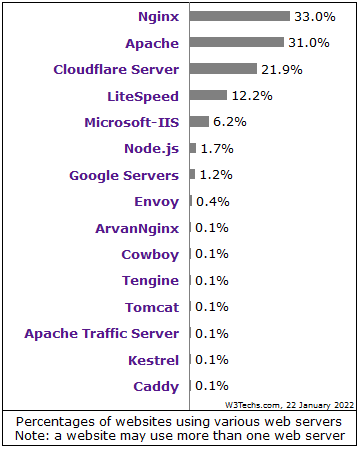
\includegraphics{images/StatistikWebserver.png}
	\caption{Benutzungsstatistiken von Webservern \cite{w3techs}}
	\label{fig:WebserverStatistik}
\end{figure}

\subsection{Apache HTTP Server}
Der Apache Webserver wurde erstmals 1995 veröffentlicht und hat sich schnell zu einem der beliebtesten Webserver entwickelt. Er unterstützt neben Unix und Linux noch eine Vielzahl an weiteren Betriebssystemen.

Der Apache Server ist modular aufgebaut, wodurch benötigte Funktionen, die der Server nicht nativ bereitstellt, durch Module importiert werden können. Das Erstellen dynamischer Webseiten wird mittels serverseitiger Skriptsprachen bewerkstelligt. Über ein Modul kann der entsprechende Interpreter in den Server integriert werden.

Beim Apache-Webserver wird ein Ansatz verfolgt, bei dem jede Clientanfrage von einem separaten Prozess oder Thread bearbeitet wird. Dadurch werden Prozesse, die Schreib- oder Leseoperationen erfordern, nacheinander abgearbeitet und es kann passieren, dass ein Request in der Warteschlange verweilen muss, bis der vorherige Request durchgeführt werden konnte. Damit man dieses Problem umgehen kann, gibt es die Möglichkeit, mehrere Single-Threading-Prozesse gleichzeitig zu starten. Diese Strategie ist jedoch mit einem hohen Ressourcenaufwand verbunden. Um dies zu vermeiden, kommen Multi-Threading-Mechanismen zum Einsatz. Für die parallele Abfrage von Clientanfragen gibt es verschiedene Multi-Processing-Module, die integriert werden können. \cite{karlstetter_2019} \cite{ionosdigitalguide_2017}


\subsection{Nginx Webserver}
Der Marktanteil von Nginx ist in den letzten Jahren kontinuierlich gestiegen, weshalb auch dieser Webserver für die Studienarbeit in Betracht gezogen wurde. Nginx wurde erstmals 2004 veröffentlicht und ist wie der Apache Server auch mit diversen Betriebssystemen kompatibel.

Wie Apache ist auch Nginx modular aufgebaut und verschiedene Funktionen können über Module bereitgestellt werden. Zu diesen Modulen gehört jedoch nicht die Option, Interpreter für eine Programmiersprache entsprechend in den Webserver zu integrieren. Es wird also ein weiterer Anwendungsserver benötigt. Für kleine Webprojekte ist das ein Mehraufwand, der nicht immer eingegangen werden muss. 

Dieser Server zeichnet sich durch eine hohe Performance aus. Dabei können eine möglichst große Anzahl an Clients gleichzeitig bedient werden und der Ressourcenverbrauch trotzdem gering gehalten. Durch die ereignisorientierte Architektur können Client-Anfragen asynchron bearbeitet werden, wodurch Arbeitsspeicher und Zeit gespart werden kann. Die Nebenläufigkeit ist realisiert, ohne dass für jede neue Verbindung ein zusätzlicher Prozess oder Thread benötigt wird. Die Stärke dieser Architektur zeigt sich bei großen Webprojekten. \cite{karlstetter_2019} \cite{ionosdigitalguide_2017}


\subsection{Fazit}
Die folgende Tabelle \ref{tab:ServerVergleich} zeigt die Unterschiede und Gemeinsamkeiten der beiden Webserver auf.

\newlength{\colWidth}
\setlength{\colWidth}{0.33\textwidth}

\begin{table}[htbp]
	\centering
	\resizebox{\textwidth}{!}{%
		\begin{tabular}{p{\colWidth}p{\colWidth} p{\colWidth}}
			\hline
			Merkmal & Apache & NGINX \\
			\hline
			Funktion & Webserver, Proxy-Server & Webserver, Proxy-Server, E-Mail-Proxy, Load-Balancer \\
			Betriebssystem & Alle unixoiden Plattformen, Windows & FreeBSD, Linux, Solaris, IBM AIX, HP-UX, macOS, Windows \\
			Lizenz & Apache License v2.0 & \acs{BSD}-Lizenz \\
			Entwickler & Apache Software Foundation & Nginx, Inc. \\
			Statische Webinhalte & Ja & Ja \\
			Dynamische Webinhalte & Ja & Nein \\
			Software-Architektur & Prozess-/threadbasiert & Eventgesteuert \\
			\hline
		\end{tabular}
	}
	\caption{Vergleich der Webserver Apache HTTP Server und Nginx Webserver}
	\label{tab:ServerVergleich}
\end{table}

Der Apache Webserver bietet eine breite Möglichkeit an Modulen, um die Software zu erweitern.
Der ausschlaggebende Grund, warum sich in diesem Projekt für den Apache HTTP Server entschieden wurde, ist die Möglichkeit Interpreter für Programmiersprachen über ein Modul direkt in den Webserver zu integrieren. Zudem muss für das Projekt nur ein Client bedient werden. Dadurch wird für das Anzeigen von dynamischen Inhalten kein separaten  Anwendungsserver benötigt. Damit bietet der Apache HTTP Server eine bequemere Lösung für kleine Websites, deren Inhalt dynamisch erzeugt wird.


\section{Framework}
Dieser Abschnitt stellt zwei verschiedene Frameworks vor, die für die Studienarbeit infrage kommen. Auch hier wird zunächst erläutert, was ein Framework ist und anschließend zwei vorgestellt, verglichen und die Nutzungsentscheidung darauf basierend begründet. 

Ein Framework ist ein Programmiergerüst. Es wird insbesondere bei komponentenbasierten und bei der objektorientierten Softwareentwicklung verwendet. Ein Framework ist kein fertiges Programm, sondern stellt den Rahmen, in der eine Anwendung erstellt werden soll, zur Verfügung. Frameworks lassen sich in Typen gliedern, wobei es nicht immer eine strikte Trennung gibt. Zu diesen Typen gehören beispielsweise  Application Frameworks oder Webframeworks.

Die beiden Frameworks, Django und Flask, die für das Projekt in Betracht gezogen wurden, gehören zu den beliebtesten Webframeworks für Python und sind für die Entwicklung von dynamischen Webanwendungen ausgelegt. \cite[195\psqq]{Java} \cite{stackoverflow} \cite{luber_2022}

\subsection{Django}
Django ist ein kostenloses Open Source Webframework und kann plattformübergreifend genutzt werden. Es folgt dem \ac{MVC} Entwurfsmuster, das auch in der Studienarbeit genutzt wird. Der Fokus von Django liegt in einer schnellen Entwicklung mit weniger Code. Mit dem Framework kommen viele bereits eingebaute Pakete, die genutzt werden können. Dazu gehört unter anderem die integrierte Anbindungen an verschiedenen Datenbanksysteme. Django hat verschiedene Mechanismen integriert, um die Sicherheit der Website zu garantieren. So können SQL Injektionen oder Cross-site Scripting ausgeschlossen werden.

Ein weiterer Vorteil von Django ist die große und aktive Community, wodurch viel Fragen schnell beantwortet werden können und es gibt es eine ausführliche Dokumentation zu dem Framework. \cite{herman_2022} \cite{luber_2022}

\subsection{Flask}
Webseiten, die Flask als Framework nutzen, sind meistens Single-Page-Webanwendungen. Flask ist im Gegensatz zu Django modular und eher minimalistisch aufgebaut. Daher muss in der Entwicklung tendenziell mit externen Bibliotheken gearbeitet werden. Man nennt Flask deshalb auch ein Mikroframework. Für die Sicherheit der Website gibt es die Flask-Security Bibliothek, die dieselben Mechanismen wie Django beinhaltet.

Aus diesen Gründen ist Flask eher für kleinere Projekte geeignet, die benutzerdefinierte Komponenten erfordern oder für das Prototyping. Die Anzahl der Webseiten, die Flask als Framework nutzen, steigt stetig weiter. Der Vorteil, warum Flask immer beliebter wird ist die Kontrolle, die man über das Projekt bekommt, indem man die Komponenten selbst bestimmen kann. \cite{herman_2022}

\subsection{Fazit}
Beide Frameworks wären für das Projekt geeignet. Die Django Community ist größer und aktiver als die von Flask. Daher gibt es mehr Informationen über Django. Jedoch wird Flask mittlerweile in mehreren Projekten genutzt. In der Tabelle \ref{tab:FrameworkVergleich} sind die wichtigsten Eigenschaften nochmals gegenübergestellt. 

\begin{table}[htbp]
	\centering
	\resizebox{\textwidth}{!}{%
		\begin{tabular}{p{\colWidth}p{\colWidth} p{\colWidth}}
			\hline
			Merkmal & Django & Flask \\
			\hline
			Use cases & mittelgroße bis große Projekte & kleine bis mittelgroße Projekte \\
			Community & große, aktive Community & kleinere Community \\
			Packages & built-in Packages & modular \\
			Performance & gut & gut \\
	
			\hline
		\end{tabular}
	}
	\caption{Vergleich der Frameworks Django und Flask}
	\label{tab:FrameworkVergleich}
\end{table}

Aufgrund der Leichtigkeit wurde sich bei den Frameworks für Flask entschieden. Da es bei der Performance keine großen Unterschiede zwischen Django und Flask gibt, ist es als Merkmal für die Entscheidung eines Frameworks nicht relevant. Für den \textbf{Sudoku Helper} wird nur eine einseitige Anwendung ohne Datenbankanbindung benötigt, wodurch Flask das geeignetere Framework ist. Auch der modulare Aufbau spricht für Flask, da nur wenige zusätzliche Pakete genutzt werden. 

Das Entwurfsmuster \ac{MVC} wird für das Framework Flask übernommen.

\section{Entwurfsmuster}
In der Studienarbeit wird für die Übersichtlichkeit ein Entwurfsmuster verwendet. Der folgende Abschnitt stellt das Entwurfsmuster und die Komponenten vor.

Wie im Abschnitt der Frameworks schon erwähnt, wird in diesem Projekt die \ac{MVC} Softwarearchitektur verwendet, damit der Programmcode eine gewisse Übersichtlichkeit behält und Kopplung reduziert wird. Dadurch lässt sich durch die Möglichkeit die einzelnen Module auszutauschen, die Skalierbarkeit erhöhen. Zudem wird das Zusammenspiel der Komponenten in einem Projekt verständlicher. Damit ist es einfacher nicht-funktionale Eigenschaften wie die Modifizierbarkeit, Wartbarkeit oder Sicherheit darzustellen und zu verstehen.  \cite[57\psq]{musch2021design}

Das Framework Django gibt das \ac{MVC} Architekturmuster vor. Da aber Flask als Framework genutzt wird, muss diese Architektur selbst implementiert werden. Im Folgenden wird das Architekturmuster mit seinen drei Komponenten kurz beschrieben.

\subsection{\acl{MVC}}
Das Ziel dieser Entwurfsarchitektur ist es, spätere Änderungen oder Erweiterungen zu vereinfachen und die Wiederverwendbarkeit der einzelnen Komponenten zu steigern. In der Abbildung \ref{fig:MVC} ist die Architektur visualisiert. Durchgezogene Linien stehen hierbei für eine direkte Assoziation und gestichelte für eine indirekte Assoziation.  \cite[57\psq]{musch2021design}

\begin{figure}[H]
	\centering
	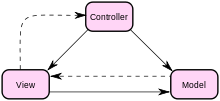
\includegraphics{images/MVC.png}
	\caption{\ac{MVC} Konzept}
	\label{fig:MVC}
\end{figure}

\subsubsection{Model}
Im Model sind die Daten enthalten, die dargestellt werden sollen. In Falle des \textbf{Sudoku Helper}s ist hier das Sudoku Board gespeichert. Dieser Teil dient zur Verwaltung und Manipulation der Daten und kommuniziert mit der View nur über den Controller.

\subsubsection{View}
In der View oder der Präsentation werden die Daten aus dem Model dargestellt. Außerdem wird in der View die Benutzerinteraktion geregelt. Die View kennt die Daten aus dem Model, soll diese aber nicht bearbeiten oder verändern. Jegliche Kommunikation mit dem Model erfolgt über den Controller.

\subsubsection{Controller}
Der Controller ist die zentrale Steuereinheit. In ihm werden das Model und die View verwaltet. Die View unterrichtet den Controller von Benutzerinteraktionen. Im Controller wird diese dann ausgewertet und gegebenenfalls das Model und die View angepasst.
